% You can write any comments you want as long as there is a percentage sign at the beginning. This won't appear in your document.

\documentclass[12pt]{article}
%	options include 12pt or 11pt or 10pt
%	classes include article, report, book, letter, thesis, with 'article' being the default layout

\usepackage{amssymb,amsmath,textcomp} %These are optional packages you can install which gives you more mathematical symbols to play with

\usepackage{graphicx,subfig,enumerate} 
\graphicspath{{img/}}


%%%%%%%%%%%%%%%%%
% CUSTOM COMMANDS



%%%%%%%%%%%%%%%%%


\title{Introduction to Vision and Robotics\\Vision Practical: Coin Counter}
\author{Dylan Angus, Matthew Martin}
\date{\today}

%%%%%%%%%%%%%%%%%%%%%%%%%%%%%%%%%%%%

% OUTLINE
% Introduction
%	a paragraph outlining the task and main ideas we used to solve it
% Methods
%	for each technique we used for background subtraction
%		list their advantages and disadvantages
%		provide images of their output
%		explain why we decided to/not to use it
%	for each technique of object segmentation/separation
%		list their advantages and disadvantages
%		provide images of their output
%		explain why we decided to/not to use it
%	explain our classifier
% Results
%	provide data (e.g. confusion matrix) for how our classifier performed under testing
%	show output images from each stage of our program
% Discussion
%	discuss the success of our program, how it could be improved, challenges/limitations we faced
% Code
%	attach all matlab code that we wrote (not anything downloaded from course website)as an appendix

%%%%%%%%%%%%%%%%%%%%%%%%%%%%%%%%%%%%%

\begin{document}
	
\maketitle

\section{Introduction}

The purpose of this practical is to develop a program in Matlab that recognises and classifies several objects in an image. These objects can be coins or other small items, and the program must segment the image, identify each of the objects, and output the total value (in pounds and pence) of the objects in the image.

All of the images are taken from a downward facing camera viewing a scene containing the objects on a static background. We were provided with a set of 14 sample images on which to train our classifier (see Figure \ref{fig:samplescene} for an example).

\begin{figure}
	\centering
	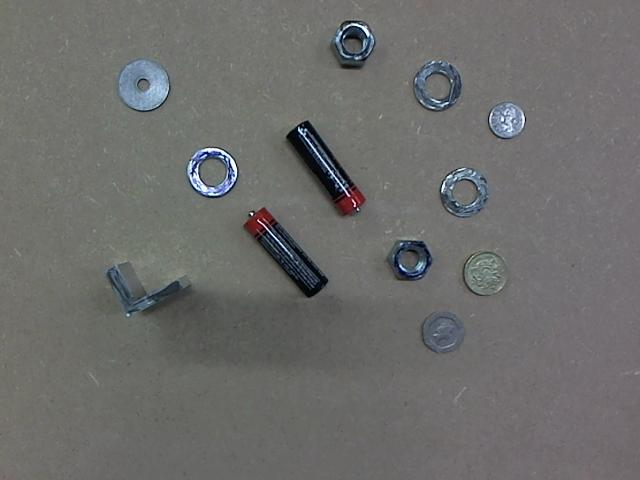
\includegraphics[width=0.75\linewidth]{02}
	\label{fig:samplescene}
	\caption{This is one of the test images given to train the classifier.}
\end{figure}

The following are the objects and associated values that may or may not be present in any given image:
\begin{itemize}
	\item one and two pound pieces
	\item 50, 20, and 5 pence pieces
	\item washer with small hole (75p)
	\item washer with large hole (25p)
	\item angle bracket (2p)
	\item AAA battery (no value)
	\item nut (no value)
\end{itemize}

We approached this problem by dividing it into three distinct stages: background segmentation, object detection, and object classification.

\section{Methods}

\subsection{Background Segmentation}

Creating a reliable algorithm that would clearly segment the background from the objects of interest in the image was the most time-consuming and challenging section of this project. We tried several different methods of background segmentation, to varying degrees of success. We ended up choosing median filter thresholding as our most successful method.

\subsubsection{Naive thresholding}

Our algorithm for creating a naive threshold can be described by the following steps:
\begin{enumerate}
	\item Attain the median values for each of the three color channels, $r,g,b$ in the given image
	\item For each pixel, if that pixel's color values are $\pm20$ from the median, label it as a background pixel. Else, label it as an object of interest.
\end{enumerate}

This method has a few advantages. It is fast, as it only requires two passes over the entire image, and there are no computationally expensive operations inside of the loop. It is simple and easy to understand. However, this method fails to accommodate for shadows in the background. It also needs to be tuned specifically to the image (the range of $\pm20$ from the medians was chosen by trial and error). Even after careful tuning, this algorithm still miss-classifies some pixels. See Figure \ref{fig:naive} for an example of the output of this method.

\subsubsection{Adaptive thresholding}

Adaptive thresholding, as opposed to naive thresholding, generates a unique threshold value for a set of sub-images inside the given image. This is meant to allow for shadows to fall on the background and still be classified as background since, the threshold is a more localized value.

This was a fairly successful method, but still had its share of disadvantages. Adaptive thresholding highlighted the edges around some of the objects rather than the objects themselves, but for others, identified the body of the object correctly. This inconsistency would cause problems when trying to classify the object. However, we never had any problems with background shadows when using this method. See the results in Figure \ref{fig:adapt}.

\subsubsection{RGB normalization}

This algorithm is meant to reduce background shadows as well by normalizing the intensity of a pixel color. It adjusts the $r,g,b$ values based on the following division:
\[r=\frac{r}{r+g+b},\hspace{5mm}g=\frac{g}{r+g+b},\hspace{5mm}b=\frac{b}{r+g+b}.\]

\subsubsection{K-means clustering}

\subsubsection{Mean-shift segmentation}

\subsubsection{Median filter thresholding}

\begin{figure}
	
	\centering
	\subfloat[naive thresholding] {
		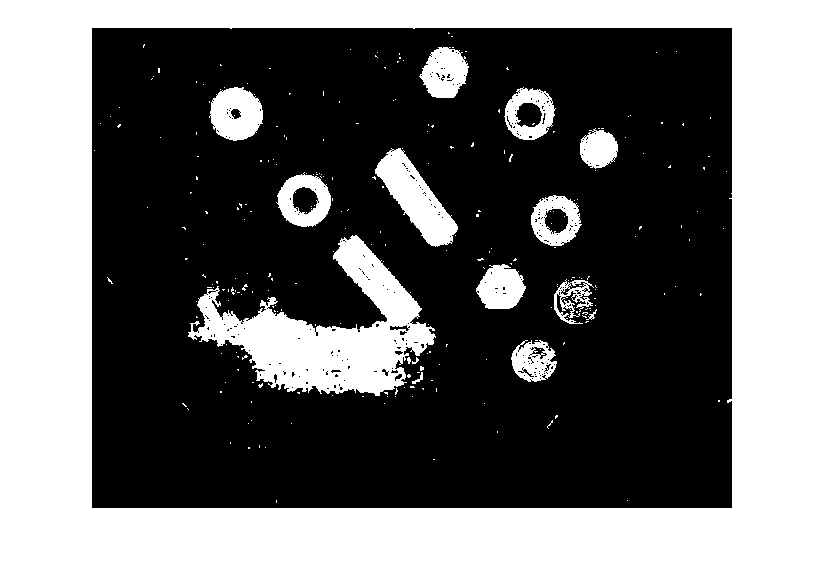
\includegraphics[width=0.5\linewidth]{naive}
		\label{fig:naive}
	}
	\subfloat[adaptive thresholding] {
		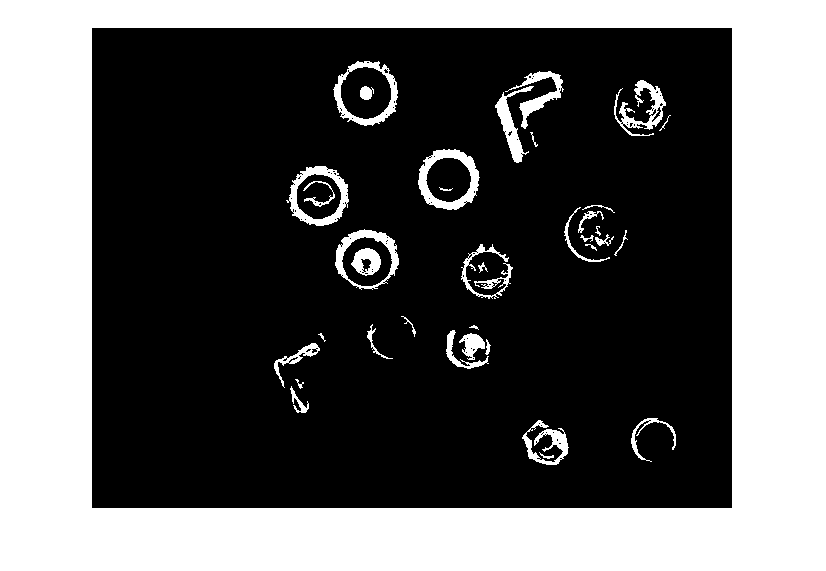
\includegraphics[width=0.5\linewidth]{adapt}
		\label{fig:adapt}
	}
	\hspace{0mm}
	\subfloat[RGB normalization] {
		
\includegraphics[width=0.5\linewidth]{norm_rgb}
		\label{fig:norm_rgb}
	}
	\subfloat[k-means classification] {
		
\includegraphics[width=0.5\linewidth]{placeholder}
		\label{fig:kmeans}
	}
	\hspace{0mm}
	\subfloat[mean-shift segmentation] {
		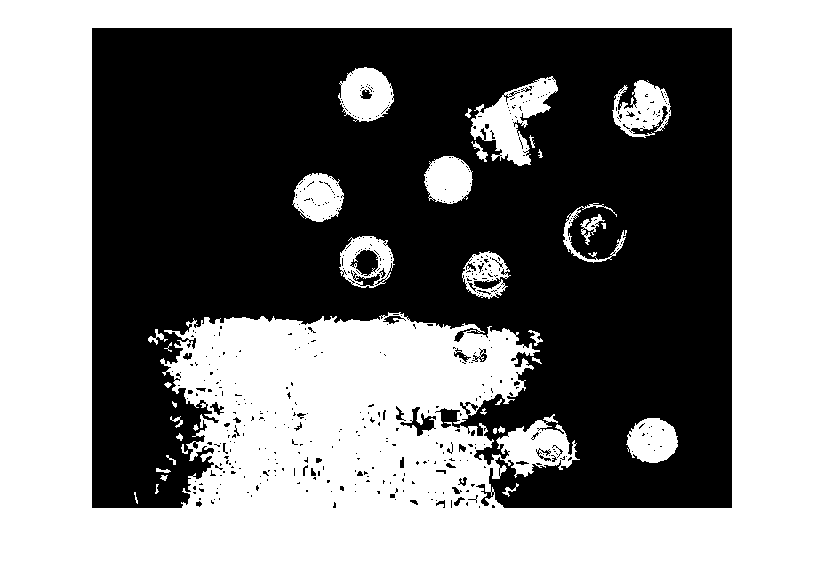
\includegraphics[width=0.5\linewidth]{mean_shift2}
		\label{fig:mean_shift}
	}
	\subfloat[median filter thresholding] {
		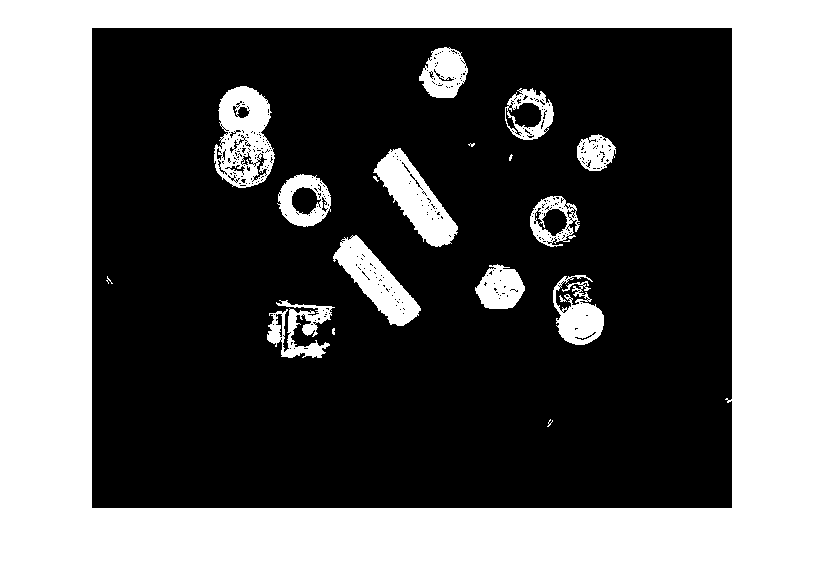
\includegraphics[width=0.5\linewidth]{median1}
		\label{fig:median}
	}
	
	\label{fig:bgseg}
	\caption{Here are the output images for the six methods of background segmentation that we tried.}
	
\end{figure}

\subsection{Object Detection}

\subsection{Classification}

\section{Results}

\section{Discussion}

\section*{Appendix}

\begin{verbatim}
	
	code can go inside these tags 
	\begin{verbatim} 
	.... 
	\ end{verbatim} (no space though)
	
\end{verbatim}


\end{document}